%%%%%%%%%%%%%%%%%%%%%%%%%%%%%%%%%%%%%%%%%
% Thesis 
% LaTeX Template
% Version 1.3 (21/12/12)
%
% This template has been downloaded from:
% http://www.latextemplates.com
%
% Original authors:
% Steven Gunn 
% http://users.ecs.soton.ac.uk/srg/softwaretools/document/templates/
% and
% Sunil Patel
% http://www.sunilpatel.co.uk/thesis-template/
%
% License:
% CC BY-NC-SA 3.0 (http://creativecommons.org/licenses/by-nc-sa/3.0/)
%
% Note:
% Make sure to edit document variables in the Thesis.cls file
%
%%%%%%%%%%%%%%%%%%%%%%%%%%%%%%%%%%%%%%%%%

%----------------------------------------------------------------------------------------
%	PACKAGES AND OTHER DOCUMENT CONFIGURATIONS
%----------------------------------------------------------------------------------------

\documentclass[11pt, a4paper, oneside]{Thesis} % Paper size, default font size and one-sided paper

\graphicspath{{./Pictures/}} % Specifies the directory where pictures are stored

\usepackage[square, numbers, comma, sort&compress]{natbib} % Use the natbib reference package - read up on this to edit the reference style; if you want text (e.g. Smith et al., 2012) for the in-text references (instead of numbers), remove 'numbers' 
\hypersetup{linkcolor=black, urlcolor=black} % Colors hyperlinks in blue - change to black if annoying
\title{\ttitle} % Defines the thesis title - don't touch this

\begin{document}

\frontmatter % Use roman pagore numbering style (i, ii, iii, iv...) for the pre-content pages

\setstretch{1.3} % Line spacing of 1.3

% Define the page headers using the FancyHdr package and set up for one-sided printing
\fancyhead{} % Clears all page headers and footers
\rhead{\thepage} % Sets the right side header to show the page number
\lhead{} % Clears the left side page header

\pagestyle{fancy} % Finally, use the "fancy" page style to implement the FancyHdr headers

\newcommand{\HRule}{\rule{\linewidth}{0.5mm}} % New command to make the lines in the title page

% PDF meta-data
\hypersetup{pdftitle={\ttitle}}
\hypersetup{pdfsubject=\subjectname}
\hypersetup{pdfauthor=\authornames}
\hypersetup{pdfkeywords=\keywordnames}

%We do not need a title page, we make one at the printers.
%----------------------------------------------------------------------------------------
%	TITLE PAGE
%----------------------------------------------------------------------------------------

%\begin{titlepage}
%\begin{center}

%\textsc{\LARGE \univname}\\[1.5cm] % University name
%\textsc{\Large Doctoral Thesis}\\[0.5cm] % Thesis type

%\HRule \\[0.4cm] % Horizontal line
%{\huge \bfseries \ttitle}\\[0.4cm] % Thesis title
%\HRule \\[1.5cm] % Horizontal line
 
%\begin{minipage}{0.4\textwidth}
%\begin{flushleft} \large
%\emph{Author:}\\
%\href{http://www.johnsmith.com}{\authornames} % Author %name - remove the \href bracket to remove the link
%\end{flushleft}
%\end{minipage}
%\begin{minipage}{0.4\textwidth}
%\begin{flushright} \large
%\emph{Supervisor:} \\
%\href{http://www.jamessmith.com}{\supname} % Supervisor name - remove the \href bracket to remove the link  
%\end{flushright}
%\end{minipage}\\[3cm]
 
%\large \textit{A thesis submitted in fulfilment of the requirements\\ for the degree of \degreename}\\[0.3cm] % University requirement text
%\textit{in the}\\[0.4cm]
%\groupname\\\deptname\\[2cm] % Research group name and department name
 
%{\large \today}\\[4cm] % Date
%\includegraphics{Logo} % University/department logo - uncomment to place it
 
%\vfill
%\end{center}

%\end{titlepage}


%Decleration page, I believe these are not normal at NTNU
%----------------------------------------------------------------------------------------
%	DECLARATION PAGE
%	Your institution may give you a different text to place here
%----------------------------------------------------------------------------------------

%\Declaration{

%\addtocontents{toc}{\vspace{1em}} % Add a gap in the Contents, for aesthetics

%I, \authornames, declare that this thesis titled, '\ttitle' and the work presented in it are my own. I confirm that:

%\begin{itemize} 
%\item[\tiny{$\blacksquare$}] This work was done wholly or mainly while in candidature for a research degree at this University.
%\item[\tiny{$\blacksquare$}] Where any part of this thesis has previously been submitted for a degree or any other qualification at this University or any other institution, this has been clearly stated.
%\item[\tiny{$\blacksquare$}] Where I have consulted the published work of others, this is always clearly attributed.
%\item[\tiny{$\blacksquare$}] Where I have quoted from the work of others, the source is always given. With the exception of such quotations, this thesis is entirely my own work.
%\item[\tiny{$\blacksquare$}] I have acknowledged all main sources of help.
%\item[\tiny{$\blacksquare$}] Where the thesis is based on work done by myself jointly with others, I have made clear exactly what was done by others and what I have contributed myself.\\
%\end{itemize}
 
%Signed:\\
%\rule[1em]{25em}{0.5pt} % This prints a line for the signature
 
%Date:\\
%\rule[1em]{25em}{0.5pt} % This prints a line to write the date
%}

%\clearpage % Start a new page

%----------------------------------------------------------------------------------------
%	QUOTATION PAGE
%----------------------------------------------------------------------------------------

\pagestyle{empty} % No headers or footers for the following pages

\null\vfill % Add some space to move the quote down the page a bit

\textit{``Thanks to my solid academic training, today I can write hundreds of words on virtually any topic without possessing a shred of information, which is how I got a good job in journalism."}

\begin{flushright}
Dave Barry
\end{flushright}

\vfill\vfill\vfill\vfill\vfill\vfill\null % Add some space at the bottom to position the quote just right

\clearpage % Start a new page

%----------------------------------------------------------------------------------------
%	ABSTRACT PAGE
%----------------------------------------------------------------------------------------

\addtotoc{Abstract} % Add the "Abstract" page entry to the Contents

\abstract{\addtocontents{toc}{\vspace{1em}} % Add a gap in the Contents, for aesthetics

The Thesis Abstract is written here (and usually kept to just this page). The page is kept centered vertically so can expand into the blank space above the title too\ldots
}

\clearpage % Start a new page

%----------------------------------------------------------------------------------------
%	ACKNOWLEDGEMENTS
%----------------------------------------------------------------------------------------

\setstretch{1.3} % Reset the line-spacing to 1.3 for body text (if it has changed)

\acknowledgements{\addtocontents{toc}{\vspace{1em}} % Add a gap in the Contents, for aesthetics

The acknowledgements and the people to thank go here, don't forget to include your project advisor\ldots
}
\clearpage % Start a new page

%----------------------------------------------------------------------------------------
%	LIST OF CONTENTS/FIGURES/TABLES PAGES
%----------------------------------------------------------------------------------------

\pagestyle{fancy} % The page style headers have been "empty" all this time, now use the "fancy" headers as defined before to bring them back

\lhead{\emph{Contents}} % Set the left side page header to "Contents"
\tableofcontents % Write out the Table of Contents

\lhead{\emph{List of Figures}} % Set the left side page header to "List of Figures"
\listoffigures % Write out the List of Figures

\lhead{\emph{List of Tables}} % Set the left side page header to "List of Tables"
\listoftables % Write out the List of Tables

%----------------------------------------------------------------------------------------
%	ABBREVIATIONS
%----------------------------------------------------------------------------------------

\clearpage % Start a new page

\setstretch{1.5} % Set the line spacing to 1.5, this makes the following tables easier to read

\lhead{\emph{Abbreviations}} % Set the left side page header to "Abbreviations"
\listofsymbols{ll} % Include a list of Abbreviations (a table of two columns)
{
\textbf{LAH} & \textbf{L}ist \textbf{A}bbreviations \textbf{H}ere \\
%\textbf{Acronym} & \textbf{W}hat (it) \textbf{S}tands \textbf{F}or \\
}

%----------------------------------------------------------------------------------------
%	PHYSICAL CONSTANTS/OTHER DEFINITIONS
%----------------------------------------------------------------------------------------

%\clearpage % Start a new page

%\lhead{\emph{Physical Constants}} % Set the left side page header to "Physical Constants"

%\listofconstants{lrcl} % Include a list of Physical Constants (a four column table)
%{
%Speed of Light & $c$ & $=$ & $2.997\ 924\ 58\times10^{8}\ \mbox{ms}^{-\mbox{s}}$ (exact)\\
% Constant Name & Symbol & = & Constant Value (with units) \\
%}

%----------------------------------------------------------------------------------------
%	SYMBOLS
%----------------------------------------------------------------------------------------

%\clearpage % Start a new page

%\lhead{\emph{Symbols}} % Set the left side page header to "Symbols"

%\listofnomenclature{lll} % Include a list of Symbols (a three column table)
%{
%$a$ & distance & m \\
%$P$ & power & W (Js$^{-1}$) \\
% Symbol & Name & Unit \\

%& & \\ % Gap to separate the Roman symbols from the Greek

%$\omega$ & angular frequency & rads$^{-1}$ \\
% Symbol & Name & Unit \\
%}

%----------------------------------------------------------------------------------------
%	DEDICATION
%----------------------------------------------------------------------------------------

\setstretch{1.3} % Return the line spacing back to 1.3

\pagestyle{empty} % Page style needs to be empty for this page

\dedicatory{For/Dedicated to/To my\ldots} % Dedication text

\addtocontents{toc}{\vspace{2em}} % Add a gap in the Contents, for aesthetics

%----------------------------------------------------------------------------------------
%	THESIS CONTENT - CHAPTERS
%----------------------------------------------------------------------------------------

\mainmatter % Begin numeric (1,2,3...) page numbering

\pagestyle{fancy} % Return the page headers back to the "fancy" style

% Include the chapters of the thesis as separate files from the Chapters folder
% Uncomment the lines as you write the chapters

% Chapter 1

\chapter{Introduction} % Main chapter title

\label{Chapter1} % For referencing the chapter elsewhere, use \ref{Chapter1} 

\lhead{Chapter 1. \emph{Introduction}} % This is for the header on each page - perhaps a shortened title

\section{Purpose/Motivation}

\section{Project context/Thesis Scope}

\section{Research questions}

\section{Research method}

\section{Thesis outline}
%\chapter{Technology} % Main chapter title

\label{Chapter2} % For referencing the chapter elsewhere, use \ref{Chapter1} 

\lhead{Chapter 2. \emph{Technology}} % This is for the header on each page - perhaps a shortened title

\section{HTML5}
HTML is a markup language for the creation of web pages. HTML describes the structure and the contents of the web page. In later years, the need for advanced styling and complex interaction with web pages has made CSS and JavaScript increasingly popular. HTML5 was created as a response to this, HTML5 is an umbrella term for creating web pages using HTML5, CSS3 and JavaScript.

HTML5 has simplified the syntax compared to earlier versions. New tags have been added to better represent the modern web page elements. Other features include media tags which greatly simplifies adding multimedia content, such as playing audio and video files. More importantly for our project is the extensive support for interactive and animated graphics through the \emph{canvas}- and \emph{svg}-tag.

The new features of HTML5 and CSS3 make it much easier to create web applications for multiple platforms and screen sizes. After the smartphone and tablet revolution creating responsive and adaptable websites has become more important. The new features included in HTML5 give large amount of flexibility with respect to the user interface and graphical visualizations.

%Is this section too short? On the other hand, is there anything more to write about CSS3 in this context?
\section{CSS3}
\emph{Cascading Style Sheets} (CSS) is a language used to describe the styling of an HTML document. Using CSS the size, color and look of HTML elements can be configured. A new feature in CSS3, which is part of HTML5, is \emph{Media Queries}. With Media Queries it is possible to specify different styling relative to the size of the screen. This functionality is useful when creating applications that target devices with different screen sizes, such as smartphones, tablets and laptops. 

%Is this section to short? Is it too stripped?
\section{JavaScript}
JavaScript is the main scripting language for web pages. It is a client-side scripting language that allows programmers to add functionality to otherwise static HTML-pages. While CSS3 takes care of the styling of HTML-elements, JavaScript is used to create customized behaviour. All modern browsers have JavaScript engines/interpreters that compile and run JavaScript code.

JavaScript is now an industry standard maintained by ECMA International. The standardized version of the script is named ECMAScript. Today ECMAScript and JavaScript are used interchangeably, and JavaScript is often used to refer to ECMAScript. Because different browsers have different implementations of the JavaScript engine, slight variations in the way JavaScript code will run on these browsers exists.

Together with HTML5 and CSS3, JavaScript is great for creating web applications that can be designed to run on both mobile and stationary devices. JavaScript has a multitude of useful open source libraries that can be used to create complex user interaction, animation, and custom graphics.

\section{Data-Driven Documents}
One of the challenges in this project is to create different visualizations to represent the activity patterns of subject. Creating custom graphics in HTML5 can be done using both the canvas- and the svg-tag. In this project SVG is used. Scalable Vector Graphics (SVG) is an image format that uses XML encoding. All popular browsers, and most mobile devices, support rendering of the svg-tags.

Creating graphics using svg-tags directly is cumbersome and time consuming. Therefore a framework that greatly simplifies this task is used. \emph{Data-Driven Documents} (D3) is an open source framework written in JavaScript. D3 supports animation and interaction with the SVG elements. This allows us to explore if animation and interactivity can improve the readability of the visualizations.

\section{activPAL}
To record the activity pattern of elderly a device called \emph{activPAL} will be used. activPAL has the shape of a small rectangle and is worn on the thigh. When the device is active it continuously records accelerometer data using an internal accelerometer. This data can be interpreted using a algorithms provided by PAL Technologies.

When the activity data has been gathered the \emph{Intelligent Activity Classification}-algorithm, provided by PAL Technologies, is used to classify the data into three different types of behaviour: sitting/laying, standing and walking. Because activPAL is worn on the thigh the accelerometer is unable to detect the difference between sitting and lying. Number of steps is also counted when walking. This data can be used to calculate how fast the person was walking.

%Is this section too short and a little strange? Maybe it should be moved to the end of the section?
Several studies have concluded that the activPAL is viable for recording and classifying activity \cite{grant2006, ryan2006, grant2008, tsavourelou}. activPAL has also been used in multiple studies for obtaining and analysing activity patterns \cite{grant2010, lord, ryan2010}.

Though this projects main focus is how to present the data and not analysis of it, the accuracy is not a huge concern. It is however important that the data presented to test subjects* reflects a realistic activity pattern. Another important factor is to show that data from a simple monitoring device can be used to create complex visualizations.
 
%\chapter{Related Products and Research} % Main chapter title

\label{Chapter3} % For referencing the chapter elsewhere, use \ref{Chapter1} 

\lhead{Chapter 3. \emph{Related Product and Research}} % This is for the header on each page - perhaps a shortened title

%We should write about the many smartphone apps that offer self-tracking.
\section{Related Products}
In 2011 a movement known as Quantified Self*\cite{quantfiedSelf} had their first conference \cite{bodyHackers}, here people shared data that they had collected about themselves width different types of devices. The goal is to gather as much information about yourself as possible, to learn about yourself through quantitative data. Members of Quantified Self* collects information about everything form sleep patterns and diets to mood and stress levels.
%Maybe make it clearer that it is an exchange of information between QS and developers?
The exchange of information within the movement between users and tool makers %Tool makers, really?
 allows for new, exciting and relevant technology to be developed. The FuelBand\cite{fuelBand}, Fitbit\cite{fitBit} are some of results of this cooperation, and both products seem to be well received by the movement. %ADD CITATION, ARTICLE NOT DONE YET. CHECK BACK SOON

\subsection{Nike+}
The Nike+ concept has existed since 2010 and is the brand name Nike uses for sports related activity tracking. %Cite here maybe
%"It started with a sensor" maybe a little to informal?
It started with a sensor in the shoe and a receiver connected to an iPod. Since then the Nike+ line has expanded into Kinect Games, sport watches and shoe implants \cite{nikeProducts}. As the product line increased so did the community around it. Every Nike+ device now requires an online profile where user can store information, create goals, and look at their history. However the Nike+ Fuelband \cite{fuelBand} is the first product aimed at monitoring the user outside of their workout, and motivating them to reach the daily activity goal

%Maybe write a little bit about their visualization of the data collected. This is probably more relevant to our project since we are creating visualization not personal informatics tools. (?)

The Fuelband\cite{fuelBand} was released in early 2012 and was the first commercial wrist worn activity monitor. The wristband contains a 3-axis accelerometer that tracks the users wrist movement. Recorded activity is converted to \emph{Nikefuel}, NikeFuel\cite{nikefuel} is a unit of measurement used by all Nike activity trackers, however there are no details on how activity is converted to NikeFuel, as the algorithm is proprietary. The wristband does calculate steps and calories burned, but the NikeFuel is the prime focus of their product line. NikeFuel does not take into account gender, height, weight, but looks purely at activity. Meaning that a mile will award the same amount of points to users of very different physiology.

The information from the Fuelband can be uploaded to an iPhone%not Android?
 or laptop which then send the information to the Nike+ servers and update the users profile. The online profile provides detailed information of the users activity, showing steps, calories burned, active time, distance travelled and average fuel. Charts can be displayed for weeks, months or years. This allows the user to track their progress and look at how often they achieve or go way above their goals.\cite{fuelbandTechSpce} 

Virtual trophies are awarded for various achievements such as gathering an X amount of NikeFuel or beating your set goal by a 100\%. These trophies can then be shared with friends or displayed on the public profile to show off your achievements. The band itself can be used to view simple information such as how far you are from your daily goal, steps taken, and calories burned. A review has reported that the NikeFuel concept can almost become an addiction and lead to doing some last minute workouts the goal in order to achieve that satisfying sensation \cite{fuelbandDcRain}
%I agree that this might be a little too specific, since we are not using this technology.
%Unsure if specific technical details should be mentioned, such as that it communicates through bluetooth etc. I figure the relevancy of these products is more on how they do things and what we can learn.

\subsection{Fitbit}
The Fitbit concept wishes to be much more involved in the subjects daily life. While the Nike+ only tracks activity, Fitbit lets the user log their sleep, food, heart rate, blood pressure and glucose. It does not specifically target exercises, but instead allows the user to track their everyday life. The product line currently consists of the Zip, One, and Aria. The Zip and One are activity trackers and will automatically update the users online profile when synced. The automatic activity trackers count only steps, but other activities and even manual labour are supported and can be entered by the user. Fitbit One is also able to track stairs climbed, hours slept and sleep quality allowing this to be automatically tracked. Aria is the Fitbit WiFi weight %"Fitbit wifi weight?
, if the device is linked to an online profile it will automatically update BMI, Weight, and body fat percentage at each weighing. Currently there are no official Fitbit devices that track blood pressure, heart rate or calorie intake, these all have to be entered manually if the user wishes to do so. There is also a journal where the user can create entries to describe their day and rate their mood. %"rate of their mood"?

Similar to the Nike+ the Fitbit allows the user to set daily goals, but as the Fitbit does not use the NikeFuel system, it enables the user to set 3 separate goals: steps taken, floors climbed, and calories burned. A daily activity breakdown is provided, this breaks the activity levels for the day into 4 categories: sedentary, lightly active, fairly active, and very active. All the goal histories can be viewed on the online profile and can be categorized into day, week, months and years. This is also applicable to other measurements such sleep, mood, blood pressure and glucose levels. 

As goals are reached Fitbit members are awarded badges. These badges are very similar to the Trophies that Nike+ awards their users. It can either be for having a very active day or lifetime achievements such as accumulating over 50,000 steps. The user can choose if he wishes these badges to be public or personal, and can be displayed on the profile if desired.

A wrist worn activity monitor known as the Fitbit Flex is slated for release in June 2013. It will have the same functionality as the Fitbit One, with the exception of an altimeter, meaning it can not measure stairs climbed. This is considered to be the greatest upcoming competitor for the Nike+ Fuelband. %So what is new with the fitbit flex, is it just a cheaper version of fitbit one?



%NB: This was written without thinking much just to get something down. Probably need a serious review.
\section{Related Research}
%I would like to kill myself.
During the CHI 2013 Workshop \cite{chi2013} one of the accepted papers discussed different approaches to visualize data from personal informatics devices. %cite here
An application called Spark was created to visualize step-count data form a FitBit trakcer. %cite here
Three different visualizations were created, based on abstract art from artists like Wassily Kandinsky and Piet Mondarian: Spiral, flora and bucket. %Should we describe the visualizations more in detail?
Though the three graphs are nice to look at, at least in the writers opinion, an evaluation of the usability and motivating factor of the visualizations in Spark is sill ongoing. 

%\chapter{Methodology} % Main chapter title

\label{Chapter4} % For referencing the chapter elsewhere, use \ref{Chapter1} 

\lhead{Chapter 4. \emph{Research Methodology}} % This is for the header on each page - perhaps a shortened title}

\section{Background}
All research methods fall into two categories: Quantitative and qualitative research \cite{realWorldResearch}. Qualitative research is suitable when one wishes to gain an understanding of an underlying phenomenon through explanations and reactions the subjects bring forward. To achieve this the researches have to interview and observe the subjects who are evaluating the object. Quantitative research are appropriate when one wishes to gain a broader understanding of a phenomenon by seeing the effects of some manipulation or activity on the phenomenon. Unlike qualitative research, quantitative research focuses on measurement, quantification and generalization of data. This in turn promotes comparison and statistical analysis of the data gathered.



\section{Focus group}
Focus group, or group interview is an informal technique that can help software developers identify the users needs and feelings about the system in question. The technique can be used both before interface design and long after implementation. 

According to Nielsen \cite{focusGroup} the focus group should have at least six participant to maintain a flowing discussion and provide different perspectives. The participants should be representative of the intended users, or be the final users themselves. Sessions normally last two hours and are run by a moderator. The moderator is responsible for keeping the discussion relevant to the session goals while letting everyone contribute and not hindering the input of ideas and comments from the participants. %Liker ikke helt den siste setningen
A single session may not be representative enough or can get sidetracked, it is therefore important to run more than one focus group.

Nielsen \cite{focusGroup} discusses two pitfalls with focus groups: Sessions are in groups therefore the participants are unable to test the system themselves, so a demo is normally provided instead. The problem with such a demo is that the participants never have to question what to do next or consider the meaning of the screen options. The second problem is that what participants say they want is not necessarily what they need, or things described by the moderator might be perceived differently by the participants. By providing concrete examples through prototypes of the technology, one can minimize this problem. 
%\chapter{Prototype} % Main chapter title

\label{Chapter5} % For referencing the chapter elsewhere, use \ref{Chapter1} 

\lhead{Chapter 5. \emph{Prototype}} % This is for the header on each page - perhaps a shortened title}

\section{Initial Graphs}

\subsection{Pie chart}
The pie chart can easily show the sum of time spend in sedentary position, standing, and walking. It is however unable to show when they occurred during the day, and for how long each activity took place. We imagine this could be used to quickly identify days with a low amount of activity, before spending time looking at more detailed visualisations.


\subsubsection{Scientific}
The first draft for a pie chart can be seen in figure \ref{fig:scientificPie}, is what we primarily think of when the word pie chart is mentioned. We have discussed if we should display percentage, time or both and how this should be implemented. Putting them next to legends, on the pie chart itself, or having it appear when a section of the pie chart is selected are all possible solutions.

Instead of using solid colours the pie chart a set of circles or "balls" can be used. Each ball represents a interval of continuous activity. So a small number of large sedentary balls represent few but long periods in a sedentary position. A ball chart visualization has more elements to take in, but help illustrate the subjects activity pattern.


\begin{figure}[h!]
	\centering
		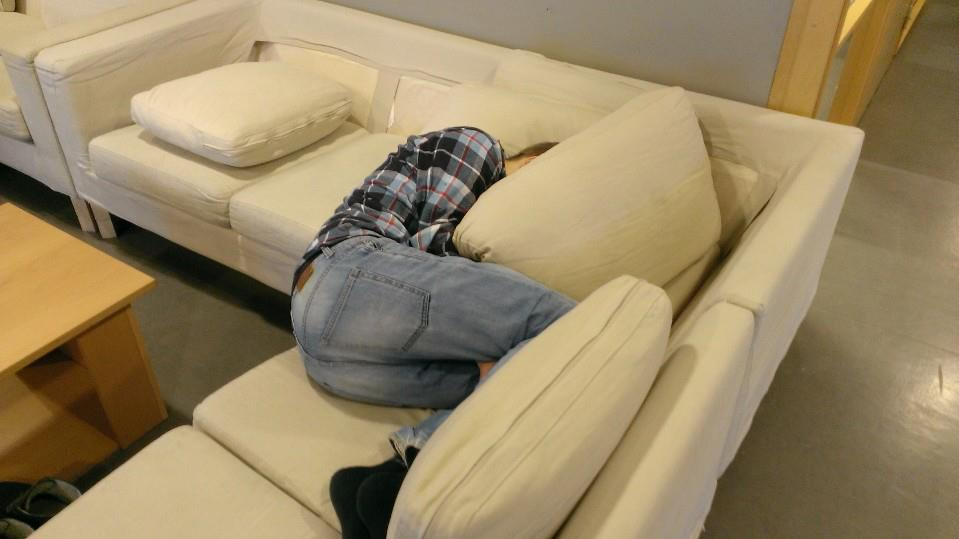
\includegraphics[width=0.5\textwidth]{placeholder.jpg}
		\caption{\footnotesize A sketch of how we envision the scientific pie chart}
		\label{fig:scientificPie}
\end{figure}

\subsubsection{Symbolic}
Our Initial approaches were very scientific, therefore our advisor suggested we think a bit more symbolic and artistic. One of the suggestions (Figure\ref{fig:symbolicPie}) was using stick figures to represent an activity. The size of each stick figure would reflect time spent in each activity, i.e a large walking figure would represent a high amount of hours walking. %SKAL VI HA TELL HE ELLER IKKE, SI NOE OM HVORFOR/HVORFOR IKKE

\begin{figure}[h!]
	\centering
		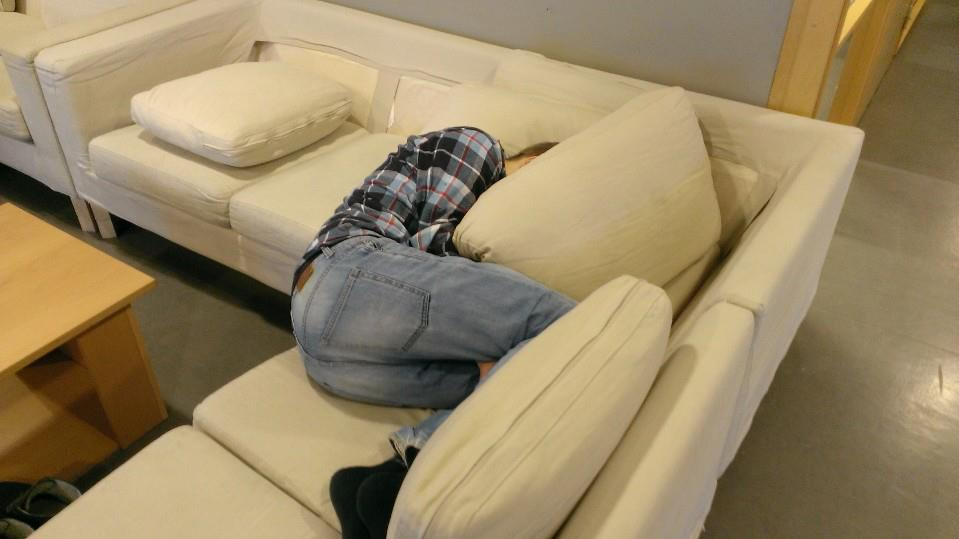
\includegraphics[width=0.5\textwidth]{placeholder.jpg}
		\caption{\footnotesize Rough drafts of a symbolic "pie chart"}
		\label{fig:symbolicPie}
\end{figure}

\subsection{Timeline}
Timeline visualisations are effective at illustrating when various activities occurred during the day. Such a bar can be used to identify points during the day where the subject is in a sedentary position for too long.

\subsubsection{Scientific}
A simple yet effective timeline was our first approach. A sketch can be seen in figure \ref{fig:simpleTimeline}. The entire day is represented by a horizontal bar where each color corresponds to an activity. A symbol can be used to highlight where sedentary time is higher than a set limit. The size of the bar would have to be quite big in order for a user to inspect some of the shorter time frames, therefore the possibility for a zoom functionality should be explored.

Instead of having a continuous scale a blocked approach can be used. The timeline would be divided into 24 blocks, each block corresponding to an hour. A gradient colour scale would be used to represent the amount of activity inside the hour block. This should make it easy to identify hours in the day where prolonged sedentary positions are present.

\begin{figure}[h!]
	\centering
		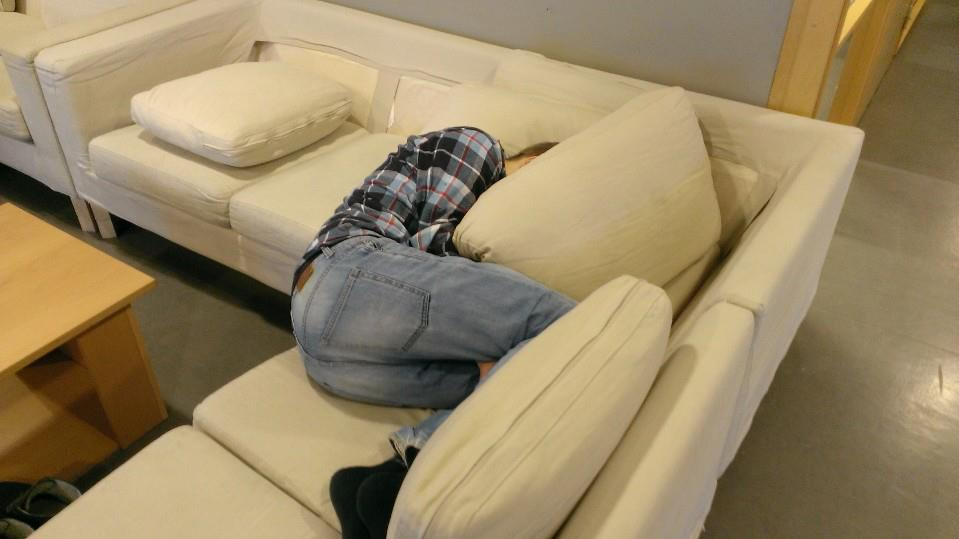
\includegraphics[width=0.5\textwidth]{placeholder.jpg}
		\caption{\footnotesize Rough drafts of a symbolic "pie chart"}
		\label{fig:simpleTimeline}
\end{figure}

\subsection{Symbolic}
An alternative approach to the standard timeline was to shape is a a clock as shown by the sketch in figure \ref{fig:clock}. Two clock would be used to split the 24 with the first clock going from 1 to 12 and the second from 13 to 24. In addition a darker colour palette could be used during hours of the night. This would deter focus away from these hours and help indicate that a high sedentary time is expected in the time period.

\begin{figure}[h!]
	\centering
		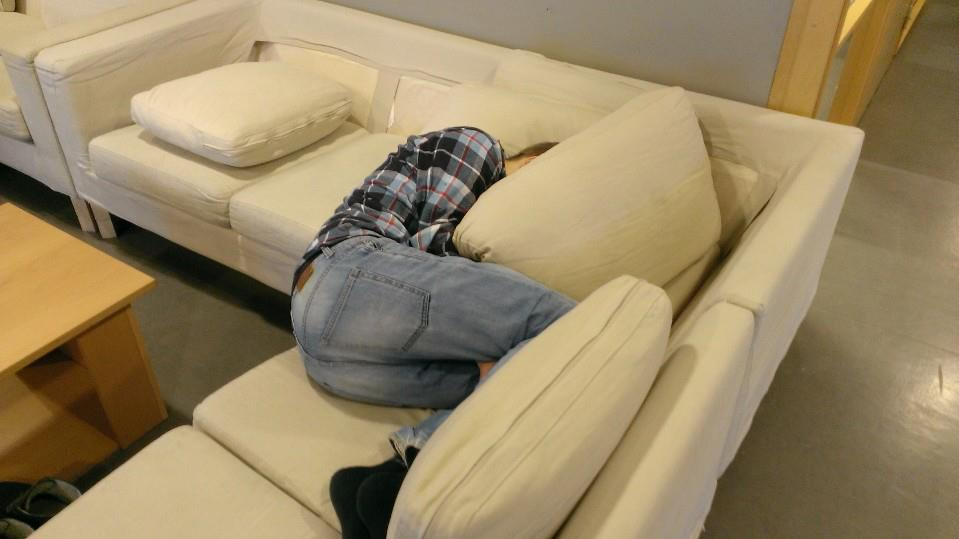
\includegraphics[width=0.5\textwidth]{placeholder.jpg}
		\caption{\footnotesize Rough drafts of a symbolic "pie chart"}
		\label{fig:clock}
\end{figure}

To really illustrate the day we came up with the idea to animate the day by using stick figures. A timeline will be drawn in real time while stick figures simultaneously perform the activities depicted on the timeline. By displaying the day gradually we hope that the subject will gain a firm understanding of their day. This means that this visualization can not be used to gain a quick overview, but is intended to be used when viewing a day for the first time.

The more motivational approach would be to replace the stick figure with an analogy or metaphor. Instead of a stick figure, a flower could be used. Activity would allowed the plant to get sunlight, making it grow. Sedentary positions would make the weather cloudy and the flower would be unaffected.



\section{Protoype goal/focus}

\section{Prototype implementation}

\section{Findings} 
%\input{./Chapters/Chapter6} 
%\input{./Chapters/Chapter7} 

%----------------------------------------------------------------------------------------
%	THESIS CONTENT - APPENDICES
%----------------------------------------------------------------------------------------

\addtocontents{toc}{\vspace{2em}} % Add a gap in the Contents, for aesthetics

\appendix % Cue to tell LaTeX that the following 'chapters' are Appendices

% Include the appendices of the thesis as separate files from the Appendices folder
% Uncomment the lines as you write the Appendices

% Appendix A

\chapter{Appendix Title Here} % Main appendix title

\label{AppendixA} % For referencing this appendix elsewhere, use \ref{AppendixA}

\lhead{Appendix A. \emph{Appendix Title Here}} % This is for the header on each page - perhaps a shortened title

Write your Appendix content here.
%\input{./Appendices/AppendixB}
%\input{./Appendices/AppendixC}

\addtocontents{toc}{\vspace{2em}} % Add a gap in the Contents, for aesthetics

\backmatter

%----------------------------------------------------------------------------------------
%	BIBLIOGRAPHY
%----------------------------------------------------------------------------------------

\label{Bibliography}

\lhead{\emph{Bibliography}} % Change the page header to say "Bibliography"

\bibliographystyle{unsrtnat} % Use the "unsrtnat" BibTeX style for formatting the Bibliography

\bibliography{Bibliography} % The references (bibliography) information are stored in the file named "Bibliography.bib"

\end{document}  